\subsection{SUBSET SUM RECONFIGURATION}

\begin{frame}{SUBSET SUM RECONFIGURATION}
  \begin{block}{Subset Sum Problem}
      Given an integer $x$ and a set of integers $S = \{a_1, a_2, \dots, a_n\}$, we wish 
      to find a subset $A \subseteq [n]$ such that $\sum_{i \in A} a_{i} = x.$
  \end{block}
   \begin{block}{SUBSET SUM RECONFIGURATION}
    Two variants : 
      \begin{enumerate}
          \setlength\itemsep{1em}
          \item Add/remove $y$, keep sum in target range. \\
          ({\footnotesize considered by Ito and Demaine, referred as SUBSET SUM RECONFIGURATION problem (SSR).}) \\ 
          
          \item Swap $y, z$ and $y + z$, keep target sum. \\
          ({\footnotesize considered by Cardinal et al., referred as $k$-move SUBSET SUM RECONFIGURATION problem ($k$-move SSR).}) 
      \end{enumerate}
    \end{block}

\end{frame}

\begin{frame}{SUBSET SUM RECONFIGURATION}
  \begin{columns}
        \begin{column}{0.5\textwidth}
            \begin{figure}
                \centering
                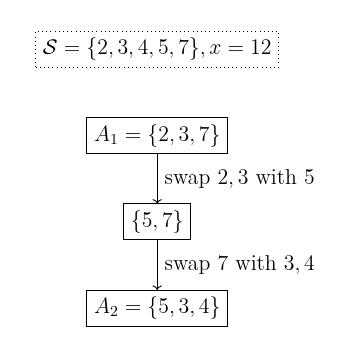
\includegraphics[width=0.9\textwidth]{img/s_1.png}
                \caption{An instance of the $k$-move SSR problem where $k = 3$.}
                \label{fig:ps}
            \end{figure}
        \end{column}
        \pause
        \begin{column}{0.5\textwidth}
            \begin{figure}
                \centering
                 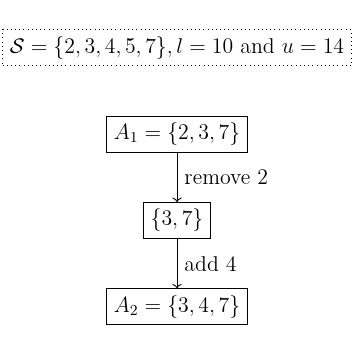
\includegraphics[width=0.9\textwidth]{img/s_2.png}
                \caption{An instance of the SSR problem.\hfill \break}
                \label{fig:circle}
            \end{figure}
        \end{column}
    \end{columns}
\end{frame}


\begin{frame}{SUBSET SUM RECONFIGURATION}
   \begin{block}{Theorem (Ito et al.)}
   The SUBSET SUM RECONFIGURATION problem is NP-hard \cite{Ito11approximabilityof}.
   \end{block}
  
   \begin{block}{Theorem (Cardinal et al.)}
   The $k$-move SUBSET SUM RECONFIGURATION Problem is PSPACE-complete for $k = 3$ \cite{cardinal_reconfiguration_2018}.
   \end{block}
\end{frame}


\begin{frame}{Geometric interpretations}
    \begin{block}{Constrained Hypercube Path problem} Given two vertices $s, t$ of the $n$-hypercube, both contained in a polytope
    $P := \{x \in \mathbb{R}^n : Ax \leq b\}$ for some $A = (a_{ij}) \in \mathbb{Z}^{d \times n}$ and $b \in \mathbb{Z}^d$, does there exist a path from $s$ to $t$ in the hypercube, all vertices of which lie in $P$?
    \end{block}
\end{frame}

\begin{frame}{Geometric interpretations}
   \begin{block}{SSR problem $\rightarrow$ Constrained hypercube path}
       \begin{itemize}
           \item Let $x \subseteq \{0,1\}^n$ Boolean variable indicating if an item is chosen or not. 
           \item The solution space of an instance of the SSR problem is represented by an $n$-hypercube. 
           \item The solutions to this given instance are the points of the $n$-hypercube that lie in the polytope $P := \{k \leq \sum_{i=1}^{n} x_{i}w_{i} \leq c\}$.
           \item The SSR problem is equivalent to the 
           Constrained Hypercube path problem where $d = 2$ since it involves exactly two linear constraints. 
           
       \end{itemize}
   \end{block}
\end{frame}

\begin{frame}{Geometric interpretation}
  \begin{block}{Example : SSR input instance}
  \begin{itemize}
      \item $\mathcal{S} = \{1,3,6\}$.
      \item The lower bound $= 1$. 
      \item The upper bound $ = 7.$
      \item $A_1 = \{6\}$ and $A_2 = \{1,3\}.$
  \end{itemize}
  \end{block}
\end{frame}


\begin{frame}{Geometric interpretation}
  \begin{block}{SSR instance $\rightarrow$ Constrained Hypercube path problem.}
    \begin{columns}
        \begin{column}{0.5\textwidth}
            \begin{figure}
            \centering
            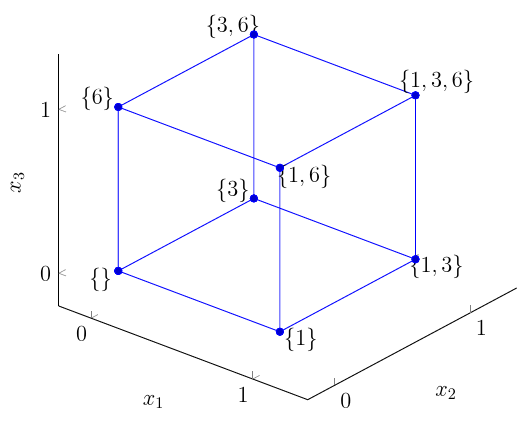
\includegraphics[width=0.9\textwidth]{img/subset_1.png}
            \caption{$n$-hypercube induced by all possible configurations of the given input SSR instance.}
            \label{fig:ps}
            \end{figure}
        \end{column}
        \pause
    \begin{column}{0.5\textwidth}
        \begin{figure}
        \centering
        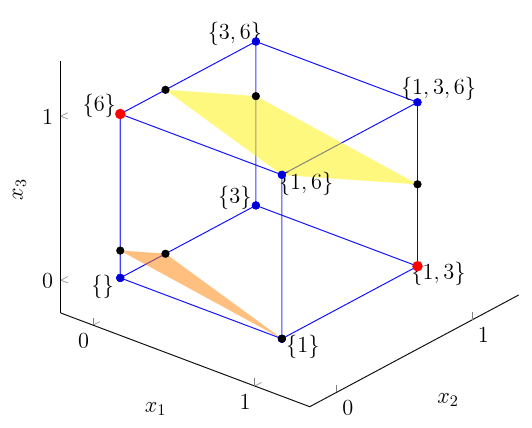
\includegraphics[width=0.9\textwidth]{img/subset_2.png}
        \caption{Polytope defined by the two linear constraints of the SSR problem.\hfill \break}
        \label{fig:circle}
        \end{figure}
    \end{column}
\end{columns}
 \end{block}
\end{frame}

\begin{frame}{Geometric interpretations}
  \begin{block}{SSR instance $\rightarrow$ Constrained Hypercube path problem.}
            \begin{columns}
                \begin{column}{0.5\textwidth}
                    \begin{figure}
                    \centering
                    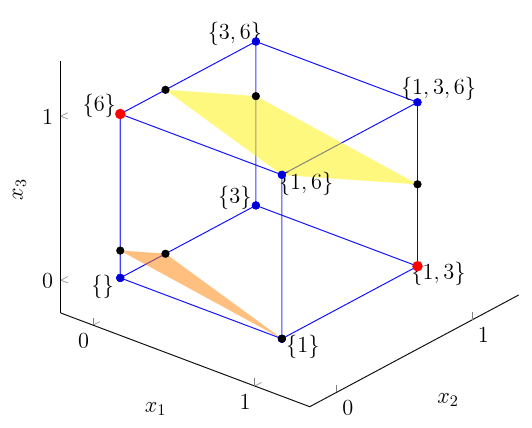
\includegraphics[width=0.9\textwidth]{img/subset_2.png}
                    \caption{Polytope defined by the two linear constraints of the SSR problem.}
                    \label{fig:ps}
                    \end{figure}
                \end{column}
                \begin{column}{0.5\textwidth}
                    \begin{figure}
                    \centering
                    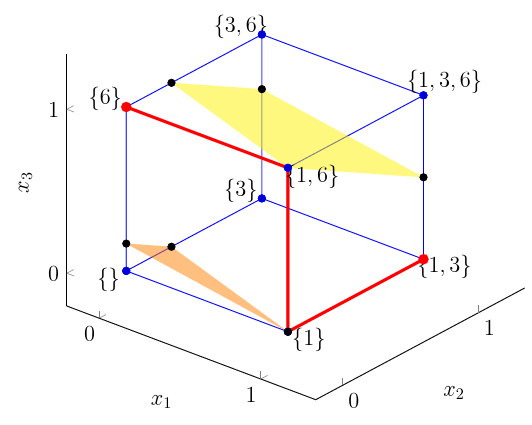
\includegraphics[width=0.9\textwidth]{img/subset_3.png}
                    \caption{Reconfiguration sequence $S$ transforming $A_1$ to $A_2$ while satisfying the capacity and treshold constraint.\hfill \break}
                    \label{fig:circle}
                    \end{figure}
                \end{column}
            \end{columns}
  \end{block}
\end{frame}

\begin{frame}{Geometric interpretations}
   \begin{block}{$k$-move SSR $\rightarrow$ Constrained hypercube path}
       \begin{itemize}
            \item Let $x \subseteq \{0,1\}^n$ Boolean variable indicating if an integer is chosen or not. 
           \item The solution space of a $k$-move SSR instance is represented by $H_n^{k}[Q]$ which is the $kth$ power of the $n$-hypercube $Q$ where two vertices are connected iff their symmetric difference is at most $k$. 
           \item The solutions to this given instance are the points of the  $H_n^{k}[Q]$ that lie in the polytope $P := \{ \sum_{i=1}^{n} x_{i}a_{i} = x\}$.
           \item The $k$-move SSR is equivalent to the Constrained Hypercube path problem where $d = 1$ since it involves exactly one linear constraint. 
       \end{itemize}
   \end{block}
\end{frame}


\begin{frame}{Geometric interpretation}
  \begin{block}{Example : $3$-move SSR input instance}
  \begin{itemize}
      \item $\mathcal{S} = \{2,3,5\}$.
      \item Target sum $x = 5.$
      \item $A_1 = \{5\}$ and $A_2 = \{2,3\}.$
  \end{itemize}
  \end{block}
\end{frame}


\begin{frame}{Geometric interpretations}
  \begin{block}{$3$-move SSR instance $\rightarrow$ Constrained Hypercube path problem.}
            \begin{columns}
                \begin{column}{0.5\textwidth}
                    \begin{figure}
                    \centering
                    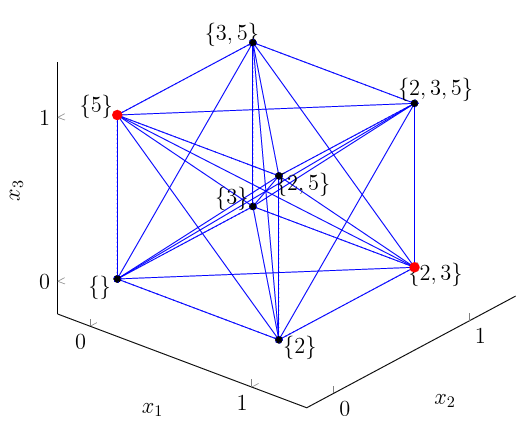
\includegraphics[width=0.9\textwidth]{img/3SSR_1.png}
                    \caption{$H_3^{3}[Q]$.}
                    \label{fig:ps}
                    \end{figure}
                \end{column}
                \begin{column}{0.5\textwidth}
                    \begin{figure}
                    \centering
                    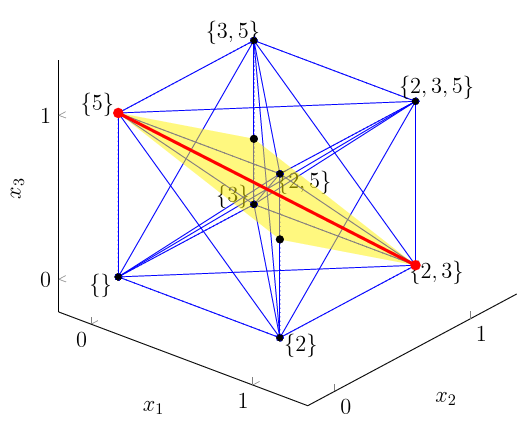
\includegraphics[width=0.9\textwidth]{img/3SSR_2.png}
                    \caption{Reconfiguration sequence $S$ transforming $A_1$ to $A_2$ while satisfying the target sum constraint.\hfill \break}
                    \label{fig:circle}
                    \end{figure}
                \end{column}
            \end{columns}
  \end{block}
\end{frame}

